\documentclass[../main.tex]{subfiles} 
\begin{document}

\section{TEORETISK GRUNNLAG}

\subsection{Systemintegrasjon}

\subsubsection{Definisjon}
Systemintegrasjon er å få to eller flere systemer til å samhandle. Det har også blitt definert som “å bringe subsystemer sammen i et system, og forsikre at subsystemene arbeider sammen i systemet”. \endnote{\url{https://en.wikipedia.org/wiki/System_integration} - 22.05.2013}

Systemintegrasjon kan gjennomføres ved å få de aktuelle systemene til å snakke med hverandre, det ene snakker til det andre, eller i situasjoner hvor det er mer enn to systemer kan det være en kombinasjon av det to løsningene. Det kan også forekomme at mellom to(eller flere) systemer blir implementert et tredje program som har som oppgave å koordinere de andre.

I systemintegrasjon snakker man ofte om cohesion, eller grad av avhengigghet. Dette refererer til hvor mye de forskjellige subsystemene er avhengige av hverandre. Man ønsker å ha så lav cohesion som mulig samtidig som at systemet må kunne utføre de oppgavene som kreves av det.

I systemintegrasjon finnes det en del forskjellige måter for programmer å samhandle. Her følger en kort beskrivelse av de vanligste metodene:

\subsubsection{Data Scraping}
Data-scraping er en teknikk som involverer bruken av software-program til å hente ut spesifikk og meningsfull data fra et annet datasett formatert for å presentere menneskeleselig data. Begrepet menneskeleselig beskriver informasjon formatert på en måte beregnet for å kunne vises til og forstås av en sluttbruker, noe som ofte innebærer at den relevante informasjonen man søker er omsluttet av irrelevant eller redundant data, eller befinner seg uforutsigbart i datasettet. Fordi datastrukturen dermed ikke egner seg for videreføring av data mellom programmer, skiller data-scraping fra syntaktisk data-analyse eller parsing som benytter seg av etablerte formateringsregler. 

Web-scraping er en mer spesifikk teknikk innen data-scraping for å lokalisere og hente ut data fra nettsider som inneholder ustrukturert data. En nettside svarer typisk med data formatert som HTML, og selve scraping-delen vil da bestå i å filtrere vekk unødvendig data, og plukke ut og sortere relevant data programmatisk.

\begin{itemize}
\item Fordeler:
	\begin{itemize}
	\item Trenger ikke tilgang til nettsidens API
	\item Krever ikke ekstra arbeid fra kildenettsiden sin side
	\item Kan innhente data fra nettsider uten å ha en avtale med kildenettside
	\end{itemize}
\item Ulemper:
	\begin{itemize}
	\item Ikke dynamisk, ved endringer til nettsidens struktur må algoritmene omskrives
	\item Kan være noe tungvint å bruke
	\item Ikke sikkert kildenettsiden tillater scraping
	\end{itemize}
\end{itemize}

Alternativer for scraping av data i Java
\begin{itemize}
\item Jsoup \endnote{\url{jsoup.org}}
\item Tagoup \endnote{\url{http://home.ccil.org/~cowan/XML/tagsoup/}}
\item HTMLUnit \endnote{\url{http://htmlunit.sourceforge.net/}}
\item Web Harvest \endnote{\url{http://web-harvest.sourceforge.net/}}
\item jArvest \endnote{\url{http://sing.ei.uvigo.es/jarvest/examples.html}}
\end{itemize}

\subsubsection{API}
Et API (Application Programming Interface) er et grensesnitt som gir eksterne brukere og applikasjoner tilgang til en annen applikasjons eller systems tjenester, funksjoner og data. Ved bruk av API kan man bygge store modulære systemer. Dette vil også si at om man vil endre funksjonaliteten på et program, så kan man endre den “indre” koden i programmet uten at det påvirker andre program som avhenger av det.

\subsubsection{Fil-dump baserte systemer}
Eldre datasystemer hadde ofte ikke tilgang på store mengder minne. Variabler og mellomlagring av data måtte derfor skrives til disk. Dette gjorde at om man ville hente inn data fra et fil-dump basert program, måtte man lese fra disse filene. Den største ulempen med denne metoden er at disk IO er veldig tregt i forhold til IO fra minne, så disse operasjonene var generelt ganske trege. Et annet problem var samtidighet mellom flere kilder når de vil lese og/eller skrive til/fra den samme kilden. Om et program skriver til en fil samtidig som et annet leser fra den, kan det oppstå feil. Dette er riktignok håndtert automatisk i nyere operativsystemer, men det kan fortsatt oppstå feil hvor et program ikke gir fra seg rettighetene til å lese/skrive til en fil.
Selv om dette er en lite brukt måte å utvikle systemer på idag, finnes det fremdeles i bruk i mange bedrifter hvor det ikke har blitt byttet ut.

\subsubsection{Fysisk oppfanging}
En mindre brukt måte å innhente data fra et system er å fysisk innhente et signal. Dette kan gjøres enten ved å omdirigere datatrafikk via et nytt punkt, eller ved å bruke en sensor som kan oppfange signalet uten å forstyrre det.

\paragraph{Kabel}
For å oppfange informasjon fra en kabel, kan man kjøre trafikken gjennom et ekstra ledd. Dette er gjerne enten en datamaskin som kopierer dataene(Pakkesniffing), og så sender den videre til sin originale destinasjon, eller en enklere mekanisk logger som man bare putter på kabelen. Disse metodene kan være helt legitime, men blir desverre ofte brukt til ulovlige formål, da de er vanskelige å oppdage.

En annen måte å innhente data fra en kabel er å måle det elektromagnetiske feltet rundt kabelen. Denne løsningen er ikke spesielt godt egnet for kompleks dataoverføring, da det ofte er mer enn en leder i en datakabel som da vil forstyrre magnetfeltet. Det er derimot fullt mulig å overvåke enkeltledere.

\paragraph{Trådløst}
Man kan lytte til trådløs kommunikasjone mellom enheter for å innhente data. Denne informasjonen er som regel kryptert, så den kan være vanskelig å dra nytte av informasjonen. Denne metoden er veldig sjeldent brukt til systemintegrasjon da den kan være både upålitelig pga. tap av signalstyrke og forstyrrelser fra andre radiosignaler i tillegg til at om man er nødt til å innhente data på denne måten er det mer praktisk å gjøre det over et kablet nettverk istedet.

\subsection{Robots.txt}
Dette er en protokoll som brukes av nettsider til å fortelle nettjenester om de få lov til å innhente data automatisk. De vanligste tjenestene som bruker denne sjekken er søkemotorer(google, yahoo etc.), men den er aktuell for alt og alle som vil innhente data fra en nettside eller tjeneste.
Protokollen kan forby tilgang til deler av sin egen mappestruktur, eller for å blokkere spesifikke tjenester(ofte blokkere søkemotorer). Det er viktig å merke seg at denne protokollen ikke aktivt blokkerer noe som helst, men fungerer som internettets trafikkskilt. Det vil si at protokollen ikke hindrer deg i å gjøre noe, men den viser om det er lov eller ikke.

\subsection{Java}
\subsubsection{Beskrivelse}
Java er et objektorientert programmeringsspråk originalt utgitt av Sun Microsystems i 1995. Det er et språk hvor alt behandles som objekter, og hvor objektene kan samhandle for å utføre oppgaver. Språket er mest kjent for sin evne til å fungere på alle plattformer uten å måtte rekompilere koden. Dette prinsippet kalles Write Once, Run Anywhere(WORA), og det var Java som var først ute med denne løsningen.
Språket er utviklet med fem hovedmål:
Det skal være enkelt, objektsorientert og kjent(ligne på andre språk)
Det skal være robust og sikkert
Det skal være plattform uavhengig
Det skal ha høy ytelse
Det skal tolkes, genereres tråder og være dynamisk i sanntid
Java brukes i dag til alt ifra til et bredt spekter av formål og til mange forskjellige typer enheter. Dette innebærer bruk som webtjenere(nettsider etc.), enkeltstående applikasjoner(normale programmer) og innebygde systemer(vaskemaskiner, kaffemaskiner etc.). 

\subsubsection{Teknisk}
Java applikasjoner, eller programmer kjører på en virtuell maskin som heter Java Virtual Machine(JVM). Dette vil si at på toppen har man applikasjonen. Denne kjører på en virtuell maskin. Dette vil si at uansett hvilken fysisk maskin applikasjonen kjører på, vil alltid maskinen se lik ut for applikasjonen. Om det gjøres systemkall til operativsystemet, oversetter den virtuelle maskinen dette for applikasjonen.

\subsubsection{Versjoner}
Det finnes per mai 2013 fire utgaver, eller versjoner av Java.
\begin{itemize}
\item Java card
\item Java Platform, Micro Edition (Java ME)
\item Java Platform, Standard Edition (Java SE)
\item Java Platform, Enterprise Edition (Java EE)
\end{itemize}

Det er differensiert mellom disse versjonene for å tilby en mer spesialisert utgave av språket til forskjellig bruk. Til normal bruk vil man bruke Java SE, men om man skal skrive et program til en enhet med begrensede maskinvare ressurser kan Java ME gi bedre ytelse. Om man skal utvikle en webserver, kan Java EE passe bedre da denne har mange innebygde funksjoner som ikke Java SE har tilgang til.

\subsubsection{Java EE / EJB}
om Enterprise Java

\subsubsection{JAX-RS}
POJO (Plain Old Java Object) 
Annotasjoner (@stateless)

\subsection{Android}
\subsubsection{Beskrivelse}
Android er et operativsystem beregnet for mobile og små enheter med berøringsskjerm. Det er verdens mest brukte operativsystem på mobile enheter, og er stadig i vekst. Mye av populariteten til Android kommer av at det er tilgjengelig på et bredt utvalg av maskinvare og i alle prisklasser. For produsentene sin del er Android populært da det er hovedsakelig åpen kildekode og dermed billig å levere med sine enheter. Mange av produsentene modifiserer også operativsystemet noe for å gjøre det til sitt eget, men dette er hovedsakelig grafiske forandringer.
Android er populært hos utviklerene da det er et mer åpent operativsystem. Dette gjør at det er lettere å utvikle applikasjoner, og at de kan bli bedre integrert i den totale brukeropplevelsen ved telefonen.

\subsubsection{Teknisk}
Android er basert på en åpen kildekode linux kjerne og er skrevet i C, C++ og Java. Alle applikasjoner som blir levert til Android er skrevet i Java og og bruker XML. Dette blir kompilert om for bruk i Android sin Dalvik virtual Machine(som er Android sin version av Java Virtual Machine).

Android applikasjoner er bygd opp av to hovedkomponenter. Disse er såkalte “aktiviteter” og “tjenester”. En aktivitet er den delen som vises på skjermen, og kjører kun så lenge den blir vist på skjermen. En typisk applikasjon består av flere aktiviteter hvor man kan navigere mellom disse.
En tjeneste er en bakgrunnsprosess som kan kjøre selv om man bytter mellom aktiviteter. Tjenestene blir ofte brukt til ting som IO og mellomlagring av globale variabler.

\subsection{Glassfish}
Glassfish er en applikasjonsserver for Java Enterprise Edition webapplikasjoner. Glassfish støtter alle Java Enterprise Edition teknologiene som: JavaServer Faces, JavaServer Pages, Enterprise JavaBeans osv. 

\subsection{JSON}

\begin{figure}[h!]
  \centering
  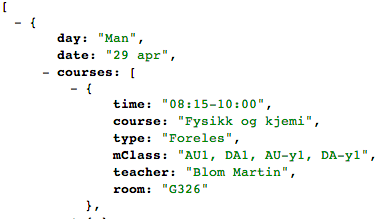
\includegraphics[width=10cm]{json.png}
  \caption{JSON data "pyntet" med en plugin for bli lettere å lese}
\end{figure}

JSON (JavaScript Object Notation) er et lettvint dataformidlingsformat som er lett å lese både av mennesker og maskiner. JSON blir ofte brukt til serialisering av data som skal sendes mellom server- og klientapplikasjoner. JSON er plattform-uavhengig.  \endnote{\url{http://www.json.org/} - 6.05.2013} \endnote{\url{http://en.wikipedia.org/wiki/Json} - 6.05.2013}

\subsection{Nettjenester}
En nettjeneste eller “web service” er en form for kommunikasjon mellom to enheter over internett. Det finst flere typer nettjenester blant annet REST-kompatible nettjenester også kalt “RESTful web services”. 
REST tjenester
REST (Representational State Transfer) er en dataoverførings-arkitektur bestående av klienter og servere. En typisk REST transaksjon er slik: klienten sender en forespørsel til serveren, serveren bearbeider forespørselen og sender tilbake data. REST bruker API ressurslinker (URI) for å representere data, eksempel på dette kan være: URL for å hente en artikkel med ID 26: http://nettside.no/tjenester/artikkel/26. 

\subsection{JSoup}
JSoup er et bibliotek for Java som blir brukt til å håndtere HTML kode fra nettsider i sanntid. Dette gjøres ved bruk av en relativt enkel API. JSoup henter ned koden fra en nettside, og så kan man navigere gjennom HTML koden for å hente ut den delen av koden man trenger. Dette er en enkel metode å web-scrape en nettside. Ulempen med denne metoden er at man må vite nøyaktig hvordan kildekoden til nettsiden man er ute etter ser ut. Man kan for eksempel hente ut info som ligger mellom spesifikke HTML notasjoner, eller man kan hente ut data ved bruk av en spesiell id. En annen funksjon er å strippe vekk alle html notasjoner, slik at man står igjen med et rent dokument.

\begin{figure}[h!]
  \centering
  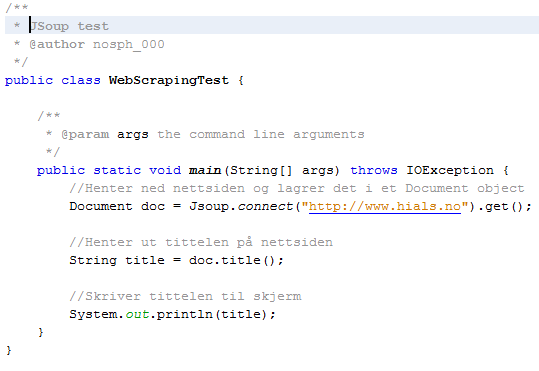
\includegraphics[width=14cm]{jsoup.png}
  \caption{Jasdasdsadsad}
\end{figure}

\subsection{Model View Controller}
\begin{wrapfigure}{r}{0.5\textwidth}
  \begin{center}
    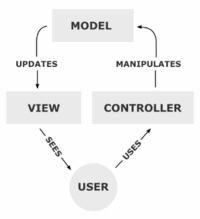
\includegraphics[width=0.3\textwidth]{mvc.png}
  \end{center}
  \caption{A gull}
\end{wrapfigure}
Model View Controller (MVC) er en arkitektur for programvare som begrenser hvilke deler av programmet brukeren samhandler med. “Model” delen består av dataen til applikasjonen (database), applikasjonslogikk, metoder og funksjoner. “View” delen består av den informasjonen fra modell-laget som er tiltenkt brukeren som for eksempel tekst, bilde, lyd osv. “Controller” delen består av håndtering av brukerens input for å styre de to andre lagene. 

\subsection{Regulære uttrykk}
Et regulært uttrykk (ofte forkortet “regex”) er en streng med karakterer som utgjør et mønster, som igjen beskriver eller matcher en eller flere strenger. Et slikt uttrykk brukes for å søke etter grupper av sammenhengende tekst, som da kan behandles på ønsket måte. Syntaksen i et regulært uttrykk varierer med implementasjonen da programmeringspråk eller programmer som har støtte for regulære uttrykk benytter seg av forskjellige prosesserings-motorer. Til tross for dette, er likevel syntaksen svært lik hvis ikke helt identisk i de fleste tilfeller.


\begin{table}
\begin{center}
\caption{This table shows some data}
  \begin{tabular}{ | p{5cm} | p{5cm} |}
    \hline
    “\textbackslash \textbackslash w” & “\textbackslash w” \\ \hline
    Java & Perl \\
    \hline
  \end{tabular}
\end{center}
\end{table}

Med unntak av spesielle karakterer, vil et regulært uttrykk beskrive en streng karakter for karakter, hvor f.eks det regulære uttrykket “regex” vil matche alle forekomster av “regex” i en annen tekststreng. De spesielle karakterene definert i syntaksen oversettes til en spesiell handling eller kan alene definere flere karakterer i en tekststreng. 

\subsection{JavaServer Faces}
JavaServer Faces (JSF) er en teknologistandard for å bygge grafiske brukergrensesnitt i serversiden, JSF blir ofte brukt i Java EE webapplikasjoner. En JSP (JavaServer Pages) fil kan inneholde standard HTML kode og JSF templates eller moduler kalt Facelets. JSF komponentene kan gjengis forskjellig på forskjellige klient-enheter. Formålet med JSF er å forenkle bygging av grafiske brukergrensesnitt for webapplikasjons-utviklere og å separere applikasjonslogikk og presentasjonslaget for modulær og teamvennlig utvikling. JSF gjør det også lettere for utviklere å kommunisere mellom applikasjonslogikken og presentasjonslaget. 

\subsection{Primefaces}
Primefaces er komponentbibliotek for JavaServer Faces som blir brukt til å lage dynamiske og funksjonsrike grafiske webgrensesnitt. Primefaces er lett å bruke, lett å implentere, har innebygd AJAX støtte og har åpen kildekode.

\subsection{AJAX}
AJAX (Asynchronous JavaScript and XML) er en gruppe teknologier brukt til å lage asynkrone klientside-funksjoner i webapplikasjoner. Dette vil si at med AJAX kan nettsider laste inn og sende data etter innlastingen av selve nettsiden, dette kan forenkle flyten i webgrensesnittet ved at brukeren kan gjøre endringer uten å måtte laste hele siden på nytt. 

\subsection{Git}
Git er et distribuert versjonskontrollsystem for programvareutvikling. Git er ideelt til teambasert programmering da det gjør det mye letter å slå sammen filer og endringer gjort av de individuelle teammedlemmene. Et git prosjekt består av en mappe der alle endringer blir lagret som revisisjoner (commits). Disse revisjonene blir organisert med full historikk slik at bidragsyterene i prosjektet kan se hvem som har gjort hvilke endringer og “rulle tilbake” endringer som ikke er ønskelige. 

\newpage

\end{document}